% !TeX root = ../thuthesis-example.tex

\chapter{对称模式挖掘算法}

本章将进一步对所提出的对称模式挖掘方法进行具体阐述。
整体来看,时间序列对称模式挖掘分为两大类,
一类是时间序列整体组成一个全局的对称模式,
另一类是对时间序列进行分段处理,由对称子序列组成的对称模式集合。
对于第一类对称模式挖掘,需要一个全局对称性度量算法和
基于时间序列数据特征的对称度阈值算法以过滤对称模式。
而若需要计算分段时间序列的对称性,
则需要在基于分段长度约束的前提下,
首先对时间序列进行分段处理,
之后通过分段对称性度量算法计算时间子序列的对称度,
然后使用由数据特征和对称度分布特征共同确定的对称度阈值
分类得到对称子序列,
最后根据挖掘数量最多不重叠对称子序列的贪心策略挖掘出对称模式。

在对时间序列的对称度进行度量之前,需要执行一步非常重要的操作,数据归一化。
这是一个在全局对称模式挖掘和分段对称模式挖掘之前都要进行的操作。由于不同来源的时间序列
数据范围往往差距很大,图~\ref{fig:data_range}展示了运输车运输过程中的经度工况时间序列和
有规律心跳过程中力感测电阻器(FSR)信号的变化时间序列,运输车经度的在
(106.89,106.9)范围内,而FSR信号在(-4000,-1000)范围内。
除了范围之外,很明显,两个数据来源的数据跨度差别也很大。
为使用统一的算法框架进行对称模式挖掘,需要对数据进行标准化处理。
对时间序列$X=\left(\left(t_{1}, x_{1}\right),\left(t_{2}, x_{2}\right), \ldots,\left(t_{n}, x_{n}\right)\right)$
的每个数据点,首先根据公式~\ref{eq:mu}计算数据点的平均值,
再根据公式~\ref{eq:sigma}计算数据点的标准差,
最后按照公式~\ref{eq:standard}对时间序列X中所有的数据点进行标准化。
使用z-score方法进行标准化,不仅在无量纲化过程中利用了所有的数据信息,
还消除了各变量在变异程度上的差异,方便提出统一的对称度阈值确定算法。
\begin{equation}
  \mu=\frac{\sum_{i=1}^{i=n} x_{i}}{n}
  \label{eq:mu}
\end{equation}
\begin{equation}
  \sigma=\sqrt[2]{\frac{\sum_{i=1}^{i=n}\left(x_{i}-\mu\right)^{2}}{n}}
  \label{eq:sigma}
\end{equation}
\begin{equation}
  y_{i}=\frac{x_{i}-\mu}{\sigma}
  \label{eq:standard}
\end{equation}
\begin{figure}
  \centering
  \subcaptionbox{挖掘机经度\label{fig:data_range-a}}
  {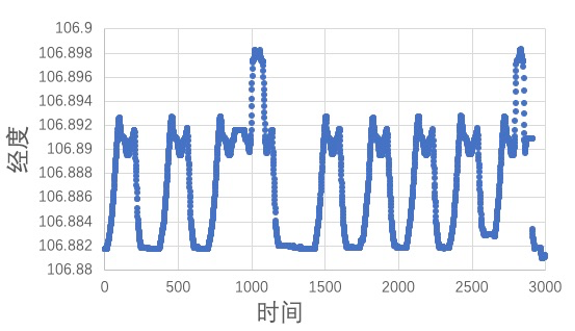
\includegraphics[width=0.43\linewidth]{truck_lo.png}}
  \subcaptionbox{心率FSR信号\label{fig:data_range-b}}
  {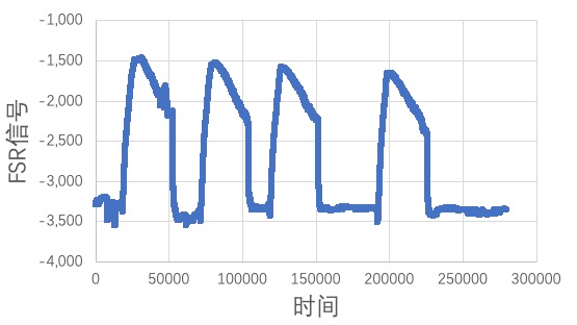
\includegraphics[width=0.43\linewidth]{heart_fsr.png}}
  \caption{多源时间序列数据分布范围}
  \label{fig:data_range}
\end{figure}

\section{全局对称模式挖掘算法}
时间序列的全局对称性指的是时间序列的所有点关于某个对称中心前后互为镜像。
全局对称模式挖掘就是要通过计算时间序列的对称度,判断时间序列是否具有对称性。
从数学意义上来说,全局对称模式挖掘算法是分段对称模式挖掘算法的子问题,
全局算法不需要以分段长度$w$作为约束,直接度量全局的对称性,并以全局对称性
在对称度阈值范围内的时间序列整体做为对称模式。
因此,全局对称模式挖掘算法由两部分构成,分别是全局时间序列对称性度量算法和
全局对称度阈值确定算法,本节将分别介绍这两种方法。
\subsection{全局时间序列对称性度量算法}

对于全局时间序列而言,使用原始时间序列和其反转时间序列的相似性来度量对称性,
是一种可行的时间序列对称性度量方法。此方法的好处是可以避免确定对称中心
的问题,但是,这种方法实际上是将时间序列对称中心两侧的子序列进行了
两次匹配,不仅降低了对称性度量算法的时间效率,还增大了对称性的度量结果。
图~\ref{fig:beijing_temp}展示了北京市自1981年至2010年月平均气温的变化,显然,
气温时间序列具有对称性。但是,经计算,原始和反转时间序列的欧式距离为
278.04,而使用本文所提出的对称性度量方法,气温时间序列的对称度仅为
7.6,更加符合真实的时间序列对称性结果。因此,本文定义了一种新的基于动态规整算法和区间动态规划思想的对称性
度量方式,既保持了动态时间规整算法准确率高、鲁棒性强的特点,
又优化了对称度的结果和计算效率。

首先从全局角度考虑对称时间序列的
匹配过程,由于不存在明确的对称中心,只能通过点和点之间的直接匹配度量
序列的对称性。由于时间序列的采集频率和位置不同,对于每个单点而言,
并不确定最佳匹配点的位置。尽管如此,如果一个时间序列是前后对称的,
那么首尾点一定是匹配的。图~\ref{fig:frontend_match}展示了
对称时间序列匹配过程的候选点,对于时间序列
$X=\left(\left(t_1,x_1 \right),\left(t_2,x_2\right),\dots,
  \left(t_n,x_n \right)\right)$而言,
第一个点$x_1$和最后一个点$x_n$是必然匹配的,但由于时间序列在
同一位置的持续时间不同,其他点如$x_2$和$x_{n-1}$等的匹配点却不是
唯一的,$x_2$可以一一对应地与$x_{n-1}$进行匹配,也可以通过扭曲时间
和$x_n$进行匹配,甚至可以与$x_{n-2},x_{n-3},\dots$等进行匹配,
而制约$x_2$与$x_k$匹配的条件不仅仅是这两点之间的距离,而是
时间序列$\left(\left(t_2,x_2 \right),\dots,\left(t_k,x_k \right)\right)$
的对称度。
\begin{figure}
  \centering
  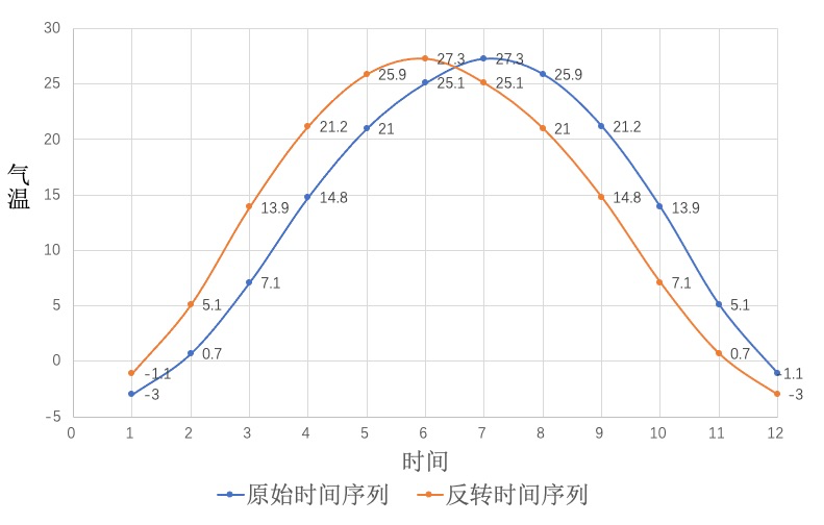
\includegraphics[width=0.86\linewidth]{beijing_temp.png}
  \caption{北京市月平均气温变化}
  \label{fig:beijing_temp}
\end{figure}

\begin{figure}
  \centering
  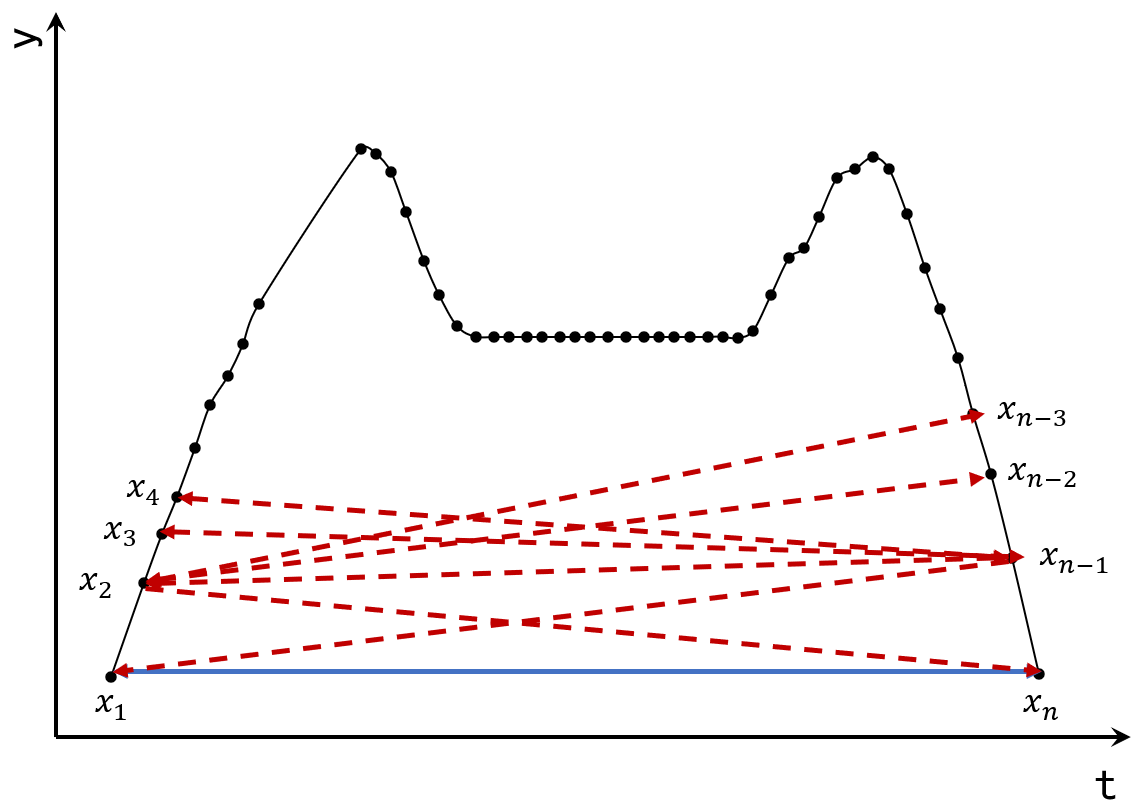
\includegraphics[width=0.76\linewidth]{frontend_match.png}
  \caption{对称时间序列首尾匹配候选点}
  \label{fig:frontend_match}
\end{figure}

接下来,本节将对时间序列的对称度算法进行标准的形式化推导。给定一条时间序列$X=\left(\left(t_1,x_1 \right),\left(t_2,x_2\right),\dots,
  \left(t_n,x_n \right)\right)$,以任意两点间的距离确立$n \times m$的
距离矩阵$D_{n \times m}$,矩阵中的每个元素由公式~\ref{eq:distance_matrix}计算而来
\begin{equation}
  D\left(i, j\right)=\left\|x_{i}-x_{j}\right\|_{w}
  \label{eq:distance_matrix}
\end{equation}

$D\left(i, j\right)$为点$p_i$与$p_j$间的距离,$i,j=1,2,\dots,n$。
显然,点$p_i$和$p_j$的匹配与$p_j$和$p_i$的匹配距离是相同的,
只是匹配顺序不同。为避免重复计算,本文只保留前点和后点的匹配,
则距离矩阵$D_{n \times m}$只需要计算反对角线以上的斜三角矩阵即可。
为了计算$X$的对称度,需要找到一条最优的匹配路径
$R_{best}=\left(r_1,r_2,\dots,r_k \right),\left⌊n/2\right⌋ \leq
  k < n$,使得$X$的累积匹配距离值达到最小, $r_k$表示该匹配路径元素在
距离矩阵中的位置,即$r_k=\left(i,j\right)_k$表示$p_i$与$p_j$之间的匹配关系,
可知$D\left(r_k \right)=D\left(i,j\right)_k$一般存在着多条匹配路径,
有效的弯曲路径$R$必须符合以下3个条件:
\begin{enumerate}
  \item 边界性:$r_{1} \in\{(i, i),(i, i+1) \mid 1 \leq i \leq n\}, \quad r_{k}=(1, n)$
  \item 单调性:给定$r_{k}=(i, j)$和$r_{k+1}=\left(i^{\prime}, j^{\prime}\right), \quad i^{\prime} \leq i, j^{\prime} \geq j$
  \item 连续性:给定$r_{k}=(i, j)$和$r_{k+1}=\left(i^{\prime}, j^{\prime}\right), \quad i^{\prime} \geq i-1, j^{\prime} \leq j+1$
\end{enumerate}

边界性是确保$R$的起点$r_1$在相似度矩阵的反对角线或者相邻斜线上,
而终点$r_k$在矩阵的右上角$\left(1,n\right)$。
单调性和连续性是为了保证匹配路径的下一个点在当前点的上方、右上方或右方。
在所有有效的路径中, 找到唯一且最优的路径使得累积匹配距离和达到最小,
公式~\ref{eq:best_route}即为优化目标:
\begin{equation}
  D(X)=\min \left\{\sum_{k=1}^{K} D\left(r_{k}\right)\right\}
  \label{eq:best_route}
\end{equation}

然而,从$r_1$到$r_k$的有效路径却是指数级的,采用暴力求解的方法不现实。
图~\ref{fig:symmetric_matrix}展示了一个时间序列在对称度矩阵上的最优
匹配路径。观察发现,路径R中的点$r_i$对于时间序列而言是由内向外匹配的。
如果$r_{k+1}$与$r_k=\left(i,j\right)$属于同一个匹配路径中的相邻点,
则$r_{k+1}$只有$(i-1, j),(i-1, j+1),(i, j+1)$这三种可能,
即$r_{k+1}$所表示的匹配范围正好包含了$r_k$的匹配范围,这种匹配顺序
符合了动态规划推导思想的无后效性。进一步,如果约定$D P(i, j)$表示时间序列
$X$的子序列$S=\left(p_{i}, p_{i+1}, \dots, p_{j}\right)$的对称度,
则该状态可以由$\{D P(i+1, j), D P(i, j-1), D P(i+1, j-1)\}$中
最小的一个推导而来,这种小区间和大区间的状态具有严格单调性的模型非常
符合区间动态规划算法思想。因此,为了求解式~\ref{eq:best_route},
利用区间动态规划方法构造一个代价矩阵$DP$, 其中每个元素通过式~\ref{eq:dp_item}得到:
\begin{equation}
  D P(i, j)=D(i, j)+\min \left\{\begin{array}{c}
    D P(i+1, j) \\
    D P(i, j-1) \\
    D P(i+1, j-1)
  \end{array}\right.
  \label{eq:dp_item}
\end{equation}

其中:$1 \leq i \leq j \leq n, D P(i, i)=0, D P(i, i+1)=D(i, i+1)$。
式~\ref{eq:dp_item}表示当前区间的匹配累积距离等于当前点的距离值加上紧邻
3个区间匹配累积距离的最小值,$D P(1, n)$便是时间序列X的最小匹配累积
代价,即对称度。得到对称度后, 为了得到最优匹配路径,
再反向以$r_k$为起点寻找匹配路径。直到$i=j$或者$i=j-1$时,
寻找过程结束,最终得到完整的匹配路径。通过累积计算匹配路径中每对匹配点之间的距离,
可以得到匹配点的距离之和,最终计算得到的$DP(1,n)$即可视为时间序列$X$的对称度。
\begin{figure}
  \centering
  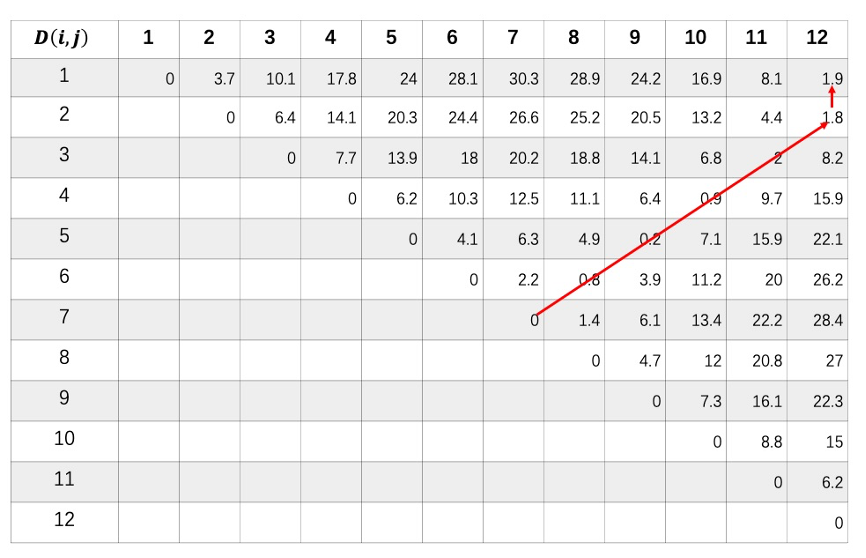
\includegraphics[width=0.86\linewidth]{symmetric_matrix.png}
  \caption{相似度矩阵最优匹配路径示意图}
  \label{fig:symmetric_matrix}
\end{figure}

\renewcommand{\algorithmicrequire}{\textbf{输入:}\unskip}
\renewcommand{\algorithmicensure}{\textbf{输出:}\unskip}

\begin{algorithm}
  \caption{全局时间序列对称性度量算法$calculate\_global\_symmetry$}
  \label{alg:global_symmetry}
  \small
  \begin{algorithmic}
    \REQUIRE 时间序列$X=\left(p_{1}, p_{2}, \dots, p_{n}\right)$
    \ENSURE 对称度$d$

    \STATE $n \leftarrow \left|X\right|$
    \STATE $i \leftarrow 1$
    \WHILE{$i \leq n$}
    \STATE $dp_{i,i} \leftarrow inf$
    \ENDWHILE

    \STATE $i \leftarrow 1$
    \WHILE{$i < n$}
    \STATE $dp_{i,i+1} \leftarrow D\left(p_{i}, p_{i+1}\right)$
    \ENDWHILE

    \STATE $len \leftarrow 3$
    \WHILE{$len \leq n$}
    \STATE $i \leftarrow len$
    \WHILE{$i \leq n-len+1$}
    \STATE $dp_{i,i+len-1} = D\left(p_{i}, p_{i+1}\right)+\min \left(dp_{i,i+len-2},dp_{i+1,i+len-1},dp_{i+1,i+len-2}\right)$
    \ENDWHILE
    \ENDWHILE
    \RETURN $dp_{1,n}$
  \end{algorithmic}
\end{algorithm}

算法~\ref{alg:global_symmetry}给出了
全局时间序列对称性度量算法的计算流程。
第1-9行初始化计算长度为1和2的时间子序列对称度,
第10-17行根据式~\ref{eq:dp_item}所示的区间动态规划算法
度量得到时间序列的全局对称度。

总结来说,本方法利用区间动态规划的算法思想,提出了一种兼顾距离相近和形状相似的时间序列对称性
度量方法,既避免了时间序列对称中心不固定带来的匹配问题,也通过异步匹配
提高了度量的准确性和健壮性,同时,因减少了重复匹配,也提高了本算法的
时间效率。尽管其渐进时间复杂度仍然为$O\left(w^{2}\right)$,
但相比于基于原始和反转时间序列的DTW距离的相似度度量算法,
减少了$50 \%$的重复匹配,并且在3.2节所述的分段时间序列对称性度量算法中
更加提升了对称子序列的计算效率。

\subsection{全局对称度阈值确定算法}
3.1.1节讲述了时间序列的全局对称性度量算法,在得到全局时间序列的对称度之后,
需要确定对称度阈值,才能判断时间序列是否具有对称性,进而挖掘出全局对称模式。
对称度阈值实际上是对时间序列进行分类,对称度在阈值范围内的
划分为对称序列,否则划分为非对称序列。因此,对称度阈值必然和时间序列本身的差异程度
密切相关。如果对称时间序列的变化比较平缓,为了将其挖掘出来,对称度阈值就需要
设定的较小。如果时间序列变化特别剧烈,相应的在进行对称时间序列匹配的过程中,
匹配点的差异可能就特别大,因此,对称度阈值也需要
设定的较小。然而,影响对称度阈值高低的关键因素不是标准差
代表的整体时间序列的差异程度,而是匹配点之间的差异程度。
图~\ref{fig:symmetry_diff}展示了标准化后正弦曲线和河北某县气温的变化时间序列,
两者都是对称时间序列。然而,尽管两者的标准差都是1,
但因为正弦时间序列完美匹配而气温时间序列匹配存在误差,
所以前者的对称度为0,而后者的对称度为0.7。
\begin{figure}
  \centering
  \subcaptionbox{标准化正弦时间序列\label{fig:symmetry_diff_sin}}
  {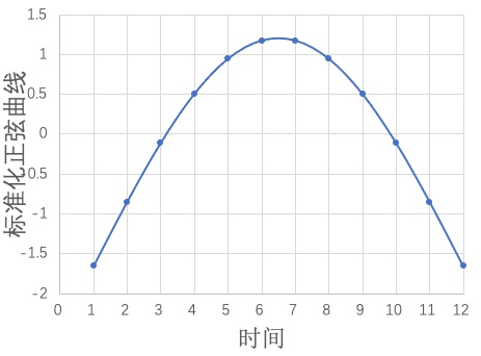
\includegraphics[width=0.43\linewidth]{symmetry_diff_sin.png}}
  \subcaptionbox{标准化气温时间序列\label{fig:symmetry_diff_temp}}
  {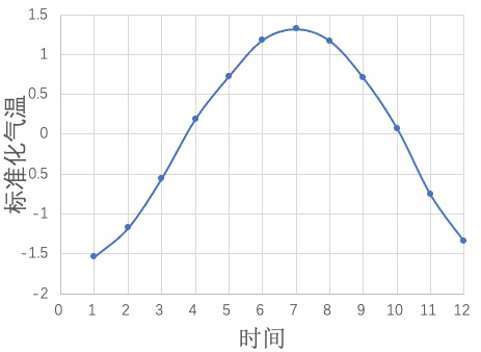
\includegraphics[width=0.43\linewidth]{symmetry_diff_temp.png}}
  \caption{多源对称时间序列对称度差异}
  \label{fig:symmetry_diff}
\end{figure}

因此,要根据时间序列点匹配的情况确定对称度阈值。然而,
根据时间序列匹配点之间的距离确定对称阈值具有极大的随机性。
对称度阈值的选取将极大地受对称性度量算法的影响。
因为对称性度量算法将决定时间序列点的匹配位置。
这样得到的对称度阈值不具有统一性,算法也不具备可迁移性。因此,
对称度阈值的确定还是需要立足时间序列本身的数据特征。
本文使用在同一个时间序列中前后相邻点的
差距作为确定对称度阈值的参考。因为对称时间序列要求前后点相匹配,
符合要求的匹配应该满足匹配点对的距离尽可能小,进而也尽量不要超过匹配点
的近邻点。式~\ref{eq:threshold1}表示时间序列近邻点距离的平均值,
可作为全局时间序列对称模式挖掘算法的对称度阈值。
对称度阈值需要统一量纲,由于不同来源时间序列对称模式的长度不一致,
因而经全局时间序列对称性度量算法计算出来的对称度
也要求其与对称模式长度的比值。算法~\ref{alg:threshold1}详述了
全局对称度阈值的计算方式。
\begin{equation}
  \theta_{1}=\frac{\sum_{i=2}^{n}\left|x_{i}-x_{i-1}\right|}{n-1}
  \label{eq:threshold1}
\end{equation}

\renewcommand{\algorithmicrequire}{\textbf{输入:}\unskip}
\renewcommand{\algorithmicensure}{\textbf{输出:}\unskip}
\begin{algorithm}
  \caption{全局对称度阈值确定算法$calculate\_global\_threshold$}
  \label{alg:threshold1}
  \small
  \begin{algorithmic}
    \REQUIRE 时间序列$X=\left(p_{1}, p_{2}, \dots, p_{n}\right)$
    \ENSURE 全局对称度阈值$\theta$

    \STATE $i \leftarrow 1$
    \WHILE{$i < \left|X\right|$}
    \STATE minus $\leftarrow$ minus $+D\left(p_{i}, p_{i+1}\right)$
    \STATE $i \leftarrow i+1$
    \ENDWHILE
    \STATE $\theta \leftarrow {\text { minus }} / (n-1)$
    \RETURN $\theta$
  \end{algorithmic}
\end{algorithm}

\section{分段对称模式挖掘算法}

3.1节介绍了全局时间序列对称度的计算,利用区间动态规划算法思想可以
计算得到全局时间序列的对称度。然而,真实的对称模式往往是聚合在一条
长时间序列之中的,其中有缺失点、异常点、噪声点等种种干扰,
接下来的挑战就是从长时间序列中挖掘出分段的对称子序列。

\subsection{分段时间序列对称性度量算法}
要对时序数据进行对称子序列的挖掘,首先要做的就是把时间序列划分成
一段一段的子序列,然后对子序列进行对称度度量。
时间序列断点检测算法是一种经典的时间子序列划分方法。
图~\ref{fig:break_detection}展示了时间序列断点检测算法的计算流程。为了检测时间序列中的关键点,
该算法采用直线对整体的时间序列数据进行拟合,如果时序数据的趋势发生了变化,
则用多条直线拟合整条时序数据。该算法使用单变量线性回归模型拟合每段时间
序列,每处理一个新数据点就重新计算多段拟合误差,利用动态规划算法全局
最大化分段效果。时间序列断点检测算法的好处是可以根据时间序列的趋势进行
关键点的判断,但是,工业时间序列中的对称模式多种多样,除去首尾点之外,
模式内部可能也存在关键点,只识别出关键点无法成功分割出对称模式。
此外,时间序列断点检测算法的复杂度高达$O\left(n^{3}\right)$,
甚至超出了对称模式挖掘算法的复杂度,在实际工业场景中不具备应用价值。
\begin{figure}
  \centering
  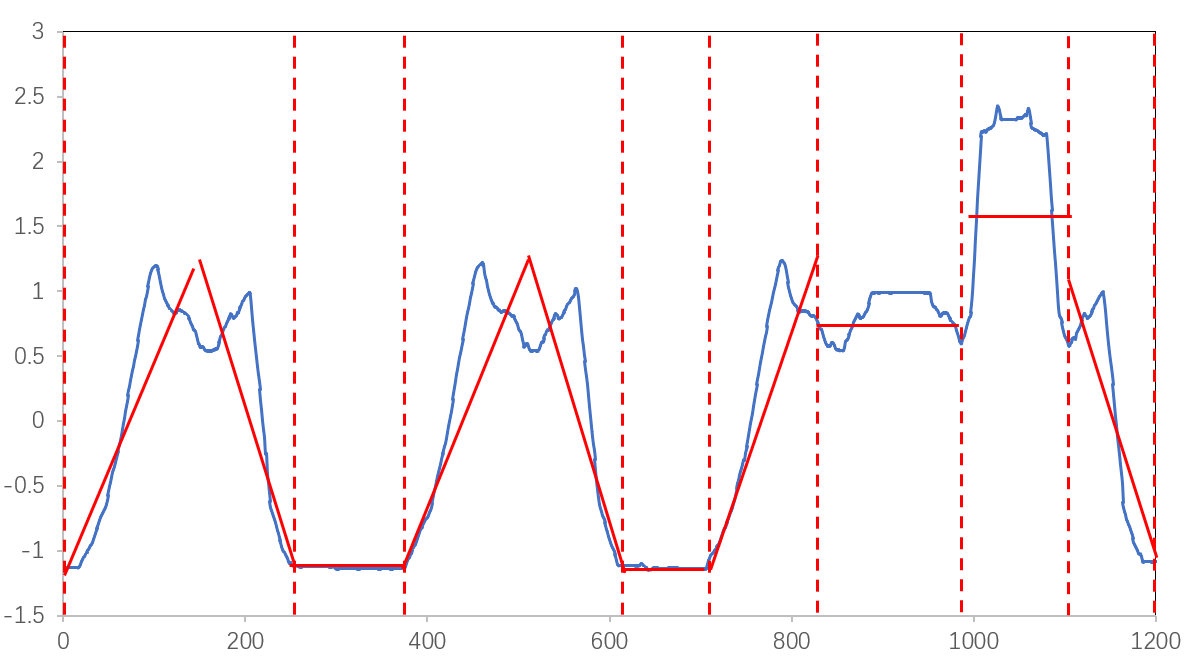
\includegraphics[width=0.86\linewidth]{break_detection.png}
  \caption{时间序列断点检测与直线拟合图}
  \label{fig:break_detection}
\end{figure}

基于此,本文选择基于滑动窗口的时间序列分段算法。滑动窗口源于网络流量控制
技术,在时间序列分析领域可以用于在特定窗口大小的子序列上执行对称度计算的
操作。通过维护一个窗口,不断向前滑动,从而划分出全部的时间序列分段。
图~\ref{fig:sliding_window}展示了使用滑动窗口将时间序列中每个长度为$w$的子序列划分出来的过程。

\begin{figure}
  \centering
  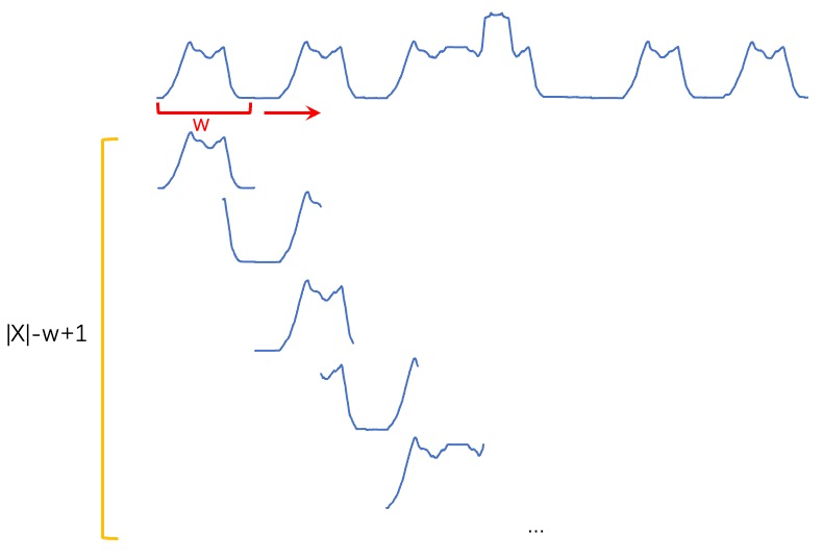
\includegraphics[width=0.86\linewidth]{sliding_window.png}
  \caption{滑动窗口时间序列分段示例}
  \label{fig:sliding_window}
\end{figure}

在滑动窗口模型中,可以直接使用3.1节所述的全局对称性度量算法计算每段时间子序列
的对称性,由于单个时间序列对称性计算的时间复杂度为$O(w^2 )$,所以全部
分段时间序列对称性度量算法的时间复杂度为$O\left(|X| \times w^{2}\right)$。
然而,利用滑动窗口和区间动态规划算法的特点可以将复杂度降低一个阶数。
考虑时间序列$X$两段长度为$w$的连续子序列$S_{i}=\left(\left(t_{i}, x_{i}\right),\left(t_{i+1}, x_{i+1}\right), \dots,\left(t_{i+w-1}, x_{i+w-1}\right)\right)$
和$S_{i+1}=\left(\left(t_{i+1}, x_{i+1}\right),\left(t_{i+2}, x_{i+2}\right), \dots,\left(t_{i+w}, x_{i+w}\right)\right)$的对称度度量,
根据式~\ref{eq:dp_item}的状态方程,时间子序列$S_i$的对称度
$D P(i, i+w-1)$由$DP(i,i+w-2)$,$DP(i+1,i+w-1)$和$DP(i+1,i+w-2)$
的最小值推导而来,而子序列$S_{i+1}$的对称度$D P(i+1, i+w)$由
$D P(i+1, i+w-1)$,$DP(i+2,i+w)$和$DP(i+2,i+w-1)$的最小值推导
而来,这两个对称度的计算都使用到了状态$DP(i+1,i+w-1)$,如果分别计算
将会产生大量的重复计算。然而,考虑到动态规划方程的无后效性,如果先计算
出时间序列$X$中所有长度为$w-1$和$w-2$的子序列对称度并保存下来,
则$S_i$和$S_{i+1}$的状态可以直接计算得到。
图~\ref{fig:fregment}展示了分段时间序列对称度推导过程,
假设时间序列$X$的长度为9,子序列长度即滑动窗口长度为5,采用窗口长度由小到大的
自底向上的推导顺序,每段子序列对称度状态都可以通过$O(1)$的复杂度计算得到,最终所有时间子序列
对称度度量的复杂度由状态个数决定,最底层长度为1的状态有$|X|$个,最顶层
长度为$w$的状态有$|X|-w+1$个,根据等差数列求和共有
$2 \times|X| \times w-w^{2}+w$个状态。
因此,分段时间序列对称度度量算法的渐进时间复杂度为$O(|X| \times w)$,
比通过原始和反转时间序列DTW距离度量对称度的$O\left(|X| \times w^{2}\right)$
效率高一个阶数。
\begin{figure}
  \centering
  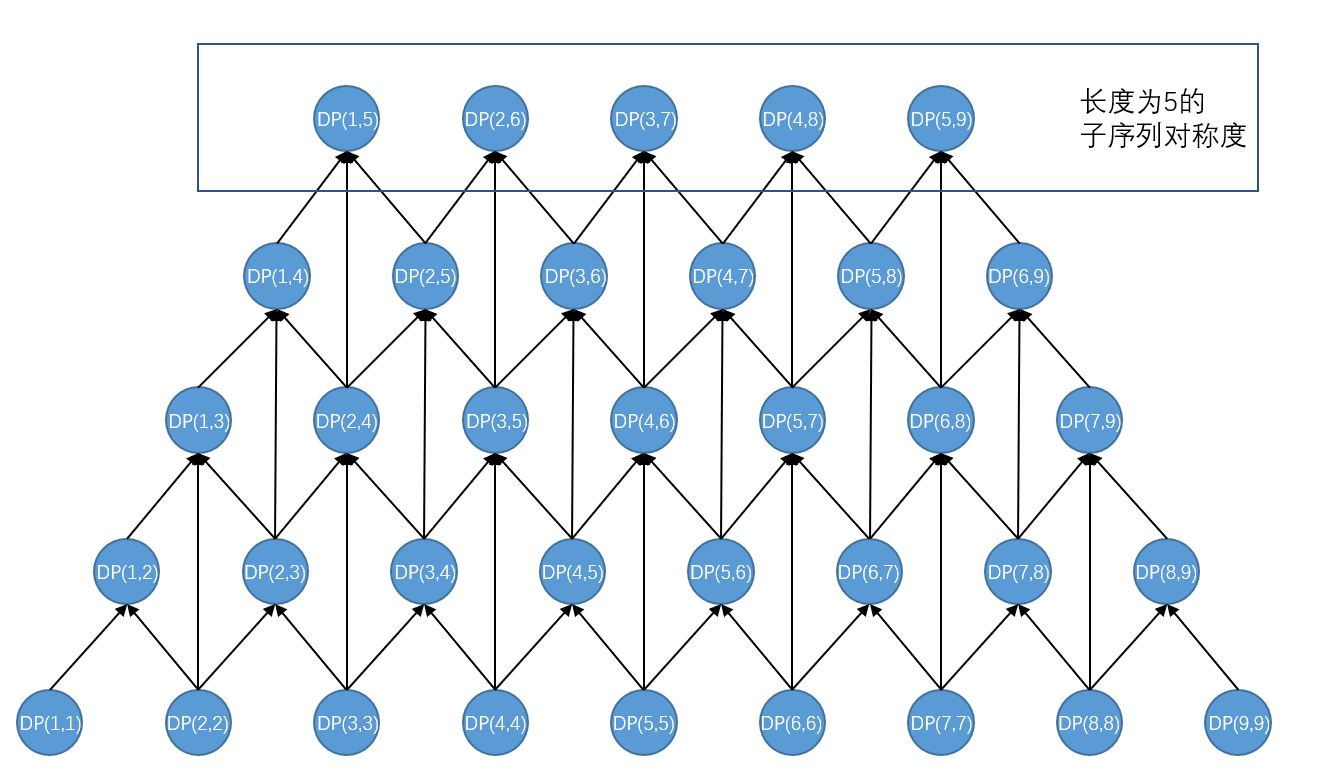
\includegraphics[width=0.86\linewidth]{fregment.png}
  \caption{分段时间序列推导流程}
  \label{fig:fregment}
\end{figure}

\subsection{分段对称度阈值确定算法}
3.2.1节讲述了分段时间序列的对称性度量算法,根据3.2.1节的算法,
给定时间序列X和子序列的长度约束$w$,可以在$O(|X| \times w)$的时间内
计算出所有的子序列对称度。然而,如果想判别出真正的对称时间子序列,
还需要至关重要的一步——确定对称度阈值。
图~\ref{fig:lontitude_symmetry}展示了运输车经度标准化处理后的时间序列和对应的分段对称度变化情况。
一般工业场景中,对称度阈值往往是由领域专家输入的。但是,并非所有的
应用场景中都能找到专业的领域专家。并且,如果对称度阈值提供的不合适,
将极大的影响对称模式的挖掘。因此,本节提出了一个基于时间序列数据特征
和对称度分布特征的对称度阈值计算方法。
\begin{figure}
  \centering
  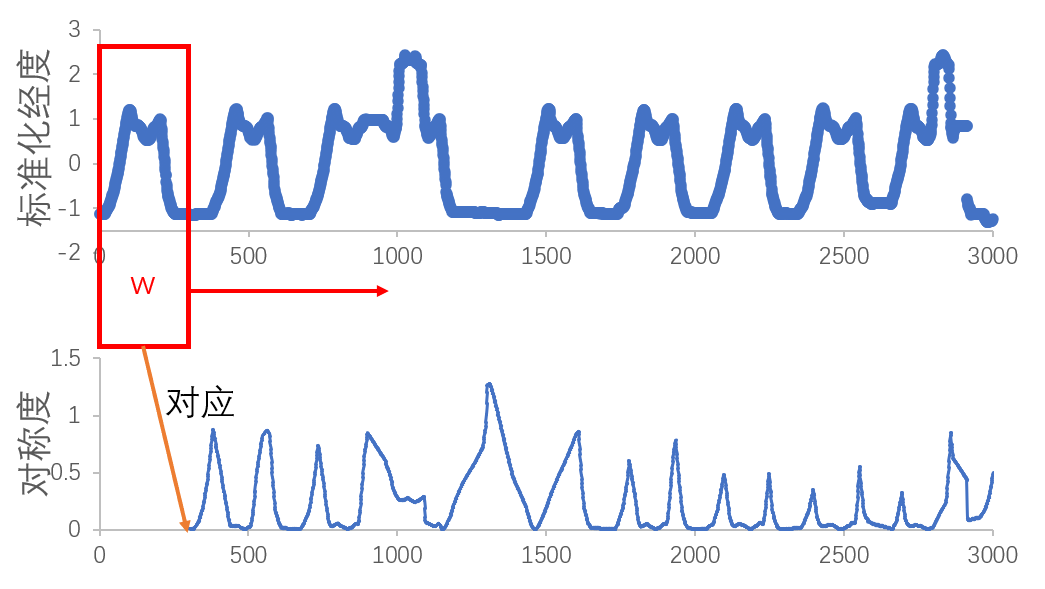
\includegraphics[width=0.86\linewidth]{std_lo_symmetry.png}
  \caption{标准化经度分段对称度变化}
  \label{fig:lontitude_symmetry}
\end{figure}

分段对称度阈值是对所有的时间子序列度量对称性,因此,除了全局对称度阈值
考虑到的时间序列数据特征,对称度自然分布同样产生阈值划分。
不同领域的时间序列数据往往具有不同种类和数量的对称模式,
相应的,其子序列对称度的数值和分布也往往有较大差异。
在概率统计中,方差用于衡量数据集中数据的偏离程度。
因此,很多算法使用方差作为度量指标变化的阈值[9]。
本文需要根据时间序列数据特征和对称度分布特征确定分段对称度阈值,
从而将子序列分为两个类别,即对称子序列和非对称子序列。
基于时间序列数据特征的阈值确定算法已在3.1.2节中详述,本节只
讨论基于分布特征的对称度阈值确定算法。

根据聚类方法[10]和自然断点分类的划分原则[11,12],
同一个类簇中数据的相似度高而不同类簇中数据的相似度低。
换言之,两个对称子序列的对称度差距应尽可能小,
而对称子序列与非对称子序列的对称度差距应尽可能大。
公式~\ref{eq:threshold2}展示了基于方差度量的对称度阈值确定原则,
其中,$DP_i$和$DP_j$均表示计算得到的子序列对称度,$\overline{D P_{i}}$̅和$\overline{D P_{j}}$
表示二者的均值。公式的最优化目标为在子序列对称度组成的集合中,
通过选择某个合适的值作为对称阈值,对称度小于该阈值的子序列为
对称子序列集合,对称度大于该阈值的子序列为非对称子序列集合,
使得对称子序列集合和非对称子序列集合的对称度方差之和最小。
图~\ref{fig:natural_break}展示了在运输车子序列对称度和挖掘机工况子序列对称度中
选择合适的自然断点,可使得对称模式和非对称模式的均值适中,
方差之和最小。综合时间序列数据特征和对称度分布的两类对称度阈值,
最终可以得到对称度阈值的完整公式,即式~\ref{eq:threshold}所示。
\begin{equation}
  \theta_{2}=\underset{x \in D P}{\operatorname{argmin}}\left(\sum_{D P_{i} \leq x}\left(D P_{i}-\overline{D P_{l}}\right)^{2}+\sum_{D P_{j}>x}\left(D P_{j}-\overline{D P_{j}}\right)^{2}\right)
  \label{eq:threshold2}
\end{equation}
\begin{equation}
  \theta=\min \left(\theta_{1}, \theta_{2}\right)
  \label{eq:threshold}
\end{equation}
\begin{figure}
  \centering
  \subcaptionbox{运煤车轨迹子序列对称度\label{fig:natural_break-a}}
  {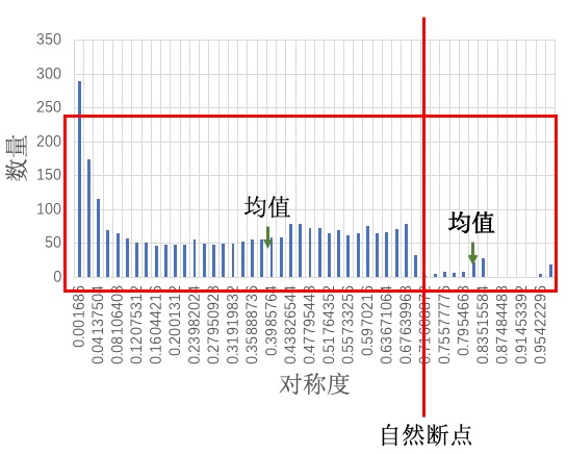
\includegraphics[width=0.43\linewidth]{natural_break-a.png}}
  \subcaptionbox{挖掘机工况子序列对称度\label{fig:natural_break-b}}
  {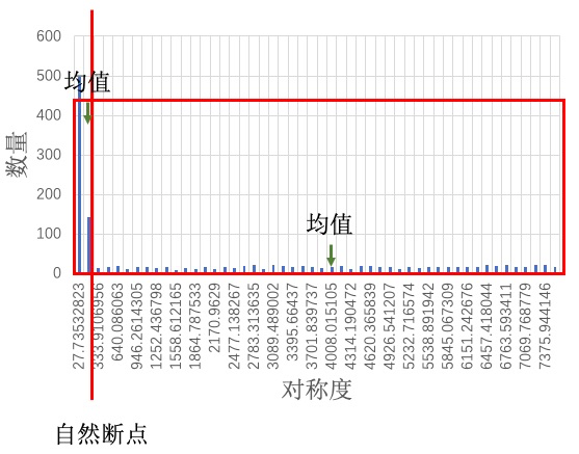
\includegraphics[width=0.43\linewidth]{natural_break-b.png}}
  \caption{运输车轨迹和挖掘机工况子序列对称度分布}
  \label{fig:natural_break}
\end{figure}

算法~\ref{alg:threshold}给出了对称度阈值的算法,考虑到
基于对称度分布的阈值确定算法需要用到
动态集合方差的计算,本文采用了流式的方差计算方法。
第1行按照大小顺序对对称度进行排序,为方差的流式计算做准备。
第2-8行根据流式算法计算前i小的对称度方差并保存到数组$l$中,从而得到
顺序排序的前缀方差数组。
第9-16行将对称度倒序排序后计算前$i$大的对称度方差并保存到数组$r$中,
由此得到倒序排序的前缀方差数组。
第17-28行通过计算前$i$小和后$n-i$大的对称度方差之和的最小值
得到基于对称度分布的阈值。
第24-35行计算时间序列相邻点距离的均值得到全局对称度阈值,
并通过和对称度分布阈值比较得到较小者,作为最终的对称度阈值。
采用这种算法得到的对称度阈值不仅考虑到了时间序列本身的特征,
还考虑到了对称度的分布,在实验结果中有良好的表现。


\renewcommand{\algorithmicrequire}{\textbf{输入:}\unskip}
\renewcommand{\algorithmicensure}{\textbf{输出:}\unskip}

\begin{algorithm}[t]
  \caption{对称度阈值划分算法$calculate\_threshold$}
  \label{alg:threshold}
  \small
  \begin{algorithmic}
    \REQUIRE 子序列对称度列表$y$,时间序列$X=\left(p_{1}, p_{2}, \dots, p_{n}\right)$
    \ENSURE 对称度阈值$\theta$

    \STATE sort$(y)$
    \STATE $a_1 \leftarrow y_1$
    \STATE $i \leftarrow 2$
    \WHILE{$i \leq \left|y\right|$}
    \STATE $a_i \leftarrow a_{i-1}+(y_i-a_{i-1})/{i}$
    \STATE $l_i \leftarrow (i-1) / (i \times i) \times(y_i-a_{i-1})^{2}+(i-1) / i \times l_{i-1}$
    \STATE $i \leftarrow i+1$
    \ENDWHILE

    \STATE reverse$(y)$
    \STATE $a_1 \leftarrow y_1$
    \STATE $i \leftarrow 2$
    \WHILE{$i \leq \left|y\right|$}
    \STATE $a_i \leftarrow a_{i-1}+(y_i-a_{i-1})/{i}$
    \STATE $r_i \leftarrow (i-1) / (i \times i) \times(y_i-a_{i-1})^{2}+(i-1) / i \times r_{i-1}$
    \STATE $i \leftarrow i+1$
    \ENDWHILE

    \STATE reverse$(r)$
    \STATE reverse$(y)$
    \STATE $d \leftarrow l_1 + r_2$
    \STATE $idx \leftarrow 1$
    \STATE $i \leftarrow 2$
    \WHILE{$i < \left|X\right|$}
    \IF{$l_i + r_{i+1} < d$}
    \STATE $d \leftarrow l_i + r_{i+1}$
    \STATE $idx \leftarrow i$
    \ENDIF
    \STATE $i \leftarrow i+1$
    \ENDWHILE
    \STATE $i \leftarrow 1$
    \WHILE{$i < \left|X\right|$}
    \STATE minus $\leftarrow$ minus $+D\left(p_{i}, p_{i+1}\right)$
    \STATE $i \leftarrow i+1$
    \ENDWHILE
    \STATE $\theta \leftarrow \min \left({\text { minus }} / (n-1), {dp_{idx}} / {n}\right)$
    \RETURN $\theta$
  \end{algorithmic}
\end{algorithm}

\subsection{挖掘分段对称模式}
计算出时间序列$X$所有在长度约束范围之内的子序列对称度之后,
可以利用贪心算法挖掘得到所有满足对称性的子序列。以斗杆外摆为例,
在挖掘过程中,存在对称子序列相互包含的情况。如图~\ref{fig:overlap}
中所示,子序列$a$、$b$、$c$均是对称子序列。由于要挖掘不重叠对称子序列,
若结果集合中选择了$a$,则不能再选择$b$和$c$。因此,
为了充分利用时间序列的信息,本文以对称子序列的数量最大值为
优化目标。根据贪心算法的思想,若上一个选择的对称子序列为$s_i$
其长度为$w$,则下一个对称子序列的贪心策略为从数据点$i+w$
开始,选择第1个长度为$w$的对称子序列, 可以保证能得到数量最多的
不重叠子序列。换言之,对于两个长度为$w$且存在重叠的时间序列,选择开始点最早的
时间序列能保证挖掘到数量最多的对称子序列。具体证明如下:假设存在3个长度为$w$的对称子序列
$A=\left(p_{i}, p_{i+1}, \dots, p_{i+w-1}\right)$,$B=\left(p_{j}, p_{j+1}, \dots, p_{j+w-1}\right)$和
$C=\left(p_{k}, p_{k+1}, \dots, p_{k+w-1}\right)$,并且$i<j<k$。若选择A序列进入
对称模式集合,则剩余对称模式可以从$p_{i+w}$之后的点进行选取。若选择B序列进入
对称模式集合,则剩余对称模式可以从$p_{j+w}$之后的点进行选取。由$i<j$可知,
$i+w<j+w$,前者的选择范围比后者更广,如果在选择B序列进入对称模式集合之后仍可选择C序列,
证明$j+w \leq k$,则$i+w$也$\leq k$,同样也可以选择A序列来替换B序列进入对称模式集合。
反之,如果选择A序列进入对称模式集合,则不一定可以由B序列替换。因此,对于长度相同的对称子序列,
选择起始时间点最早的序列能保证挖掘出最多的对称模式。

\begin{figure}
  \centering
  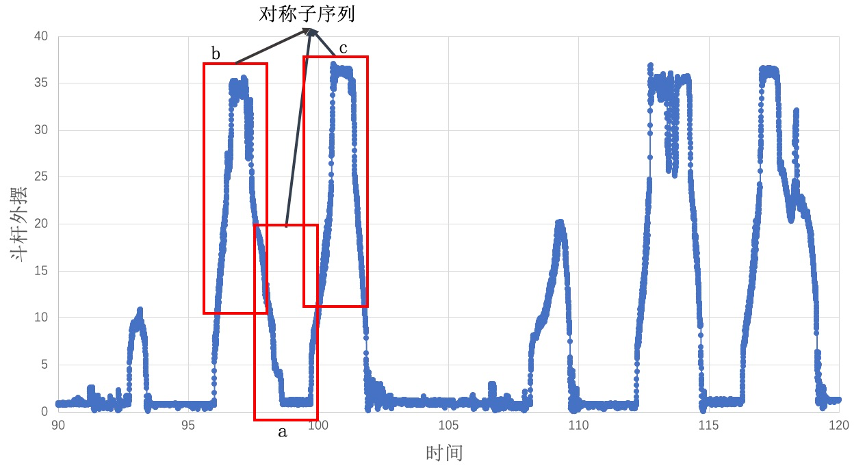
\includegraphics[width=0.86\linewidth]{symmetric_overlap.png}
  \caption{对称时间序列反映重叠现象的案例}
  \label{fig:overlap}
\end{figure}

本文根据上述对称模式挖掘方法提出了相应的具体算法,
如算法3.2所示。第1-19行根据第3.2节提出的对称度计算方式
计算了给定时间长度约束下所有子序列的对称度,第20行根据算法~\ref{alg:threshold}的计算方式
确定了对称度阈值,第21-30行根据贪心策略
计算出数量最多的不重叠对称子序列。由前述定义可知,第1-19行计算子序列对称度的时间复杂度为$O(|X| \times w)$,
第20行自然断点的确定和不重叠对称子序列的挖掘均只需要$O(|X|)$的时间。
因此,本算法的整体时间复杂度为$O(|X| \times w)$,其效率远远高于直接利用
DTW 计算的$O\left(|X| \times w^{2}\right)$,为后续的数据分析提供数据基础。
\renewcommand{\algorithmicrequire}{\textbf{输入:}\unskip}
\renewcommand{\algorithmicensure}{\textbf{输出:}\unskip}

\begin{algorithm}[t]
  \caption{时间序列对称模式挖掘算法$calculate\_symmtric\_pattern$}
  \label{alg:symmetric_pattern}
  \small
  \begin{algorithmic}
    \REQUIRE 时间序列$X=\left(p_{1}, p_{2}, \dots, p_{n}\right)$,长度约束$w$
    \ENSURE 对称模式$Q$

    \STATE $i \leftarrow 1$
    \WHILE{$i \leq \left|X\right|$}
    \STATE $dp_{i,i} \leftarrow inf$
    \ENDWHILE

    \STATE $i \leftarrow 1$
    \WHILE{$i < \left|X\right|$}
    \STATE $dp_{i,i+1} \leftarrow D\left(p_{i}, p_{i+1}\right)$
    \ENDWHILE

    \STATE $len \leftarrow 3$
    \WHILE{$len \leq \left|X\right|$}
    \STATE $i \leftarrow len$
    \WHILE{$i \leq \left|X\right|-len+1$}
    \STATE $dp_{i,i+len-1} = D\left(p_{i}, p_{i+1}\right)+\min \left(dp_{i,i+len-2},dp_{i+1,i+len-1},dp_{i+1,i+len-2}\right)$
    \ENDWHILE
    \ENDWHILE

    \STATE $i \leftarrow 1$
    \WHILE{$i \leq \left|X\right|-w+1$}
    \STATE $y_i=dp_{i,i+w-1}$
    \ENDWHILE
    \STATE $\theta = calculate\_threshold\left(y,X\right)$

    \STATE $i \leftarrow 1$
    \WHILE{$i \leq \left|X\right|-w+1$}
    \IF{$dp_{i,i+w-1}/w \leq \theta$}
    \STATE 把$S=\left(p_{i+1}, p_{i+2}, \dots, p_{i+w-1}\right)$放入对称子序列集合$Q$
    \STATE $i \leftarrow i+w$
    \ELSE
    \STATE $i \leftarrow i+1$
    \ENDIF
    \ENDWHILE
    \RETURN $Q$
  \end{algorithmic}
\end{algorithm}

\section{实验与验证}
本节将会对上面提出的时间序列对称模式挖掘算法进行实验验证和结果分析工作。具体而言,主要包括对3.1节提出的全局时间序列对称性度量算法进行结果对比和验证;对3.2节提出的对称性阈值算法进行准确性评估;对整体时间序列对称模式挖掘算法框架进行准确率评估和性能对比。
\subsection{实验环境}
本文试验所使用的环境如下表~\ref{tab:experiment_enviroment}所示

\begin{table}
  \centering
  \caption{实验环境介绍}
  \begin{tabular}{ll}
    \toprule
    实验环境     & 具体参数                          \\
    \midrule
    操作系统     & macOS 版本 10.15.5                \\
    处理器       & 2.4 GHz 四核Intel Core i5         \\
    内存         & 16 GB 2133 MHz LPDDR3             \\
    固态硬盘     & 256GB                             \\
    代码语言     & Python                            \\
    集成开发环境 & PyCharm 2020.1(Community Edition) \\
    \bottomrule
  \end{tabular}
  \label{tab:experiment_enviroment}
\end{table}

实验所使用的数据集,一方面来自UCR提供的时间序列数据集,另一方面来自真实应用场景的时间序列数据。UCR中每类数据集重的时间序列长度都相同,且经过了标准化操作,方便在同一量纲下使用对称模式挖掘算法进行计算。真实的数据集来自传感器采集的工业大数据,其中每条时间序列都包含多个工况信息,且都未进行标准化,对称模式挖掘有一定难度。针对不同实验对于数据的要求,本文选择合适的数据集进行实验,具体的数据集信息将在实验过程中进行详述。

\subsection{全局时间序列对称性度量效果评估实验}
由于时间序列的数据值是连续数据,具有一定的随机性和波动性,不同于对称字符串,现有研究中并不存在一个明确统一的对称性度量算法。因此,本文基于全局时间序列的数据特征,提出了一种基于区间动态规划和全局匹配的对称性度量算法。为了检测对称性度量算法的效果,本文在UCR数据集中选择了两个具有明显全局对称性的时间序列数据集和两个不具有全局对称性的时间序列数据集,
这4个数据集的详细介绍如表~\ref{tab:experiment_dataset}所示。

在这4个数据集中,GunPointAgeSpan的时序数据表示的一套完整的持枪动作,而UMD的时间序列表示的是实验室信号合成数据,两者都具有对称的物理意义。而GestureMidAirD1和MixedShapes分别是手势轨迹和由普通二维形状转换而来的时间序列数据,不具有对称性。分别对这两组包含正负样本的数据集进行实验,可以验证本文全局对称性度量算法的有效性。为保证正负样本的数据条数大致相同,不会出现数据倾斜问题,本文通过采样保证了对称数据集和非对称数据集的时间序列条数均为147。

\begin{table}
  \centering
  \caption{实验数据集介绍}
  \begin{tabular}{ccccc}
    \toprule
    数据集名称      & 来源         & 类型 & 数据条数 & 长度 \\
    \midrule
    GestureMidAirD1 & 3D手势轨迹   & 运动 & 47       & 361  \\
    GunPointAgeSpan & 完整举枪动作 & 运动 & 135      & 150  \\
    MixedShapes     & 二维形状转换 & 图像 & 100      & 1024 \\
    UMD             & 信号合成     & 模拟 & 12       & 150  \\
    \bottomrule
  \end{tabular}
  \label{tab:experiment_dataset}
\end{table}

本文为全局时间序列对称性度量算法设置了两个算法作为对照组实验,
其一为利用原始和反转时间序列相似性度量对称性的方法,
另一个是通过对称中心两侧子序列的相似性度量对称性的方法。
由于时间序列数据的连续性和不稳定性,不同类型时间序列数据的对称中心
不确定,因此,本文选用时间序列的几何中心作为其对称中心。
此外,正如2.4节所述,时间序列相似性度量算法种类多样,
仅基于形状的相似性度量方法就远不止一种。本文选择了包括基于
曼哈顿距离、欧式距离、DTW距离和FastDTW距离在内的4种相似性
度量方法,其中每种方法都可以用来为对照组的两个算法提供相似性度量
计算。表~\ref{tab:experiment_algorithm}对本实验涉及到的9种时间序列
对称性度量算法进行了介绍。
由于不同度量方法的计算方式不同,不同数据集的时间序列长度
也不同,为了在同一量纲上进行比较,在通过全局对称性度量算法和
其他相似性度量算法得到时间序列的全局对称度之后,需要再计算其
与时间序列长度的比值得到单点对称度,作为最终统一衡量时间序列
对称性的值。
\begin{table}
  \centering
  \caption{实验算法介绍}
  \begin{tabular}{ll}
    \toprule
    算法名称          & 计算方式                            \\
    \midrule
    symmetry          & 基于全局时间序列对称性度量算法      \\
    manhattan         & 基于原始和反转时间序列的曼哈顿距离  \\
    euclidean         & 基于原始和反转时间序列的欧式距离    \\
    dtw               & 基于原始和反转时间序列的DTW距离     \\
    fastdtw           & 基于原始和反转时间序列的FastDTW距离  \\
    center\_manhattan & 基于中心点两侧时间序列的曼哈顿距离   \\
    center\_euclidean & 基于中心点两侧时间序列的欧式距离     \\
    center\_dtw       & 基于中心点两侧时间序列的DTW距离     \\
    center\_fastdtw   & 基于中心点两侧时间序列的FastDTW距离 \\
    \bottomrule
  \end{tabular}
  \label{tab:experiment_algorithm}
\end{table}

图~\ref{fig:symmetry_compare}展示了在两个对称数据集上,
不同对称性度量算法计算得到的对称度结果。经过对比可以发现,
本文所提出的全局时间序列对称性度量算法(symmetry算法)
计算得到的对称度总是最小的,
不仅小于基于原始和反转时间序列的相似性度量对称性的算法,也小于基于中心点
两侧时间序列相似性度量对称性的算法。对于相同的对称度阈值,本算法可以挖掘出
数量尽可能多的对称时间序列和对称模式。除此之外,从本结果中还可以看出,
尽管GunPointAgeSpan和UMD数据集的时间序列具有物理意义上的对称性,而且
时间序列的长度相同,甚至都经过了标准化处理,但其对称度的分布范围仍然相差甚大。
以symmetry算法为例,在GunPointAgeSpan数据集上度量135条时间序列得到的平均对称度
是3.85,而在UMD数据集上度量12条时间序列得到的平均对称度仅为0.01,不同
来源的数据集因为数据特征的差别其对称度阈值差距较大,这为对称模式的挖掘也带来了困难,
从侧面证明了本文提出的对称度阈值算法的重要性。
\begin{figure}
  \centering
  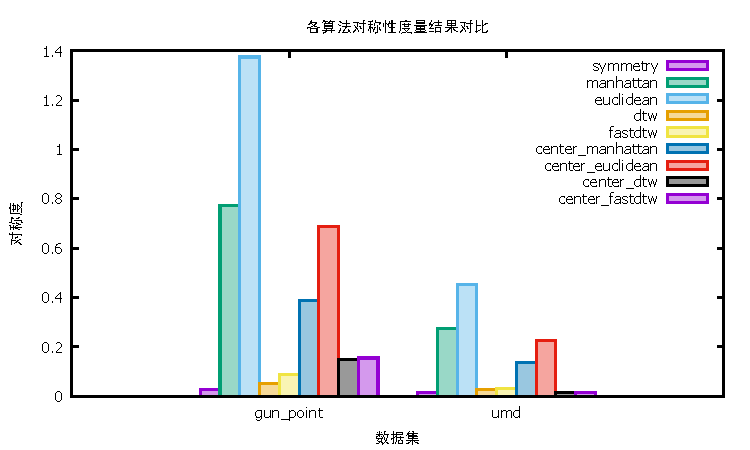
\includegraphics[width=0.86\linewidth]{symmetry.pdf}
  \caption{对称数据集不同算法的对称性度量结果}
  \label{fig:symmetry_compare}
\end{figure}

由于对全局时间序列进行对称性度量不存在时间子序列,无法利用子序列对称度
的分布确定第二类阈值,只能通过时间序列数据特征确定第一类阈值,作为
过滤对称时间序列的指标。在全局对称性度量算法的效果实验中,本文以精确率,
召回率和F值作为效果的评价指标。在4个数据集中,GunPointAgeSpan和UMD数据集
具有对称性,而MixedShapes和GestureMidAirD1数据集没有对称性。
在实验过程中,本文把对称模式标记为正类(positive),把非对称模式标为负类(negative)。
当算法在对称数据集中发现对称模式时,这类时间序列用TP表示。当算法
在对称数据集中发现非对称模式时,这类时间序列用FN表示。当算法
在非对称数据集中发现对称模式时,这类时间序列用FP表示。当算法
在非对称数据集中发现非对称模式时,这类时间序列用TN表示。
基于以上四类情况,可以定义时间序列对称模式挖掘算法的
精确率(Precision)和召回率(Recall)和F值。
其中,精确率又叫查准率,定义为在所有被预测为正的样本中,
实际为正样本的概率,在本实验中的含义是预测为对称模式的时间序列中有多少是真正的对称时间序列,
式~\ref{eq:precision}表示了精确率的计算方式。召回率又叫查全率,定义为在所有真实为正
的样本中,预测为正样本的概率,在本实验中的含义是
真实为对称模式的时间序列中有多少被预测为了对称时间序列。
式~\ref{eq:recall}表示了召回率的计算方式。F值的定义是准确率和召回率的加权平均数,
为平衡准确率和召回率,本文选择F1值作为F值度量结果,式~\ref{eq:f1}表示了
F1值的计算方式。
\begin{equation}
  Precision=\frac{TP}{TP+FP}
  \label{eq:precision}
\end{equation}
\begin{equation}
  Recall=\frac{TP}{TP+FN}
  \label{eq:recall}
\end{equation}
\begin{equation}
  F1=\frac{2 \times Precision \times Recall}{Precision+Recall}
  \label{eq:f1}
\end{equation}

\begin{figure}
  \centering
  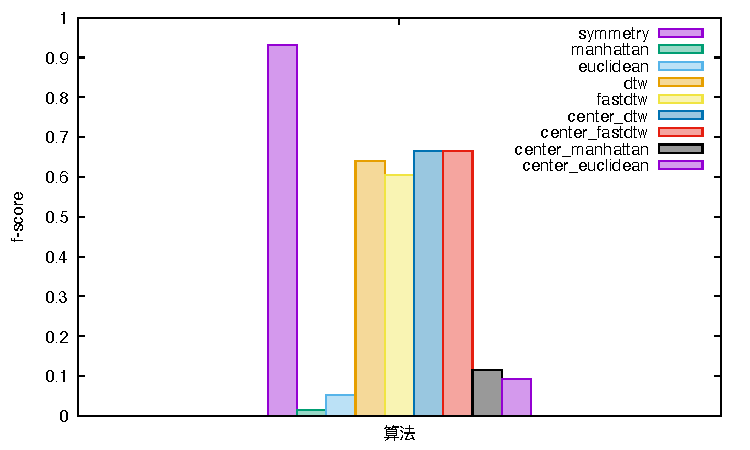
\includegraphics[width=0.86\linewidth]{f-score.pdf}
  \caption{不同对称模式挖掘算法的F-Score度量结果}
  \label{fig:fscore_compare}
\end{figure}

为了综合评价算法的挖掘效果,本文选用F值表示算法的对称模式挖掘效果。
因为精确率是挖掘出的对称模式中真正对称模式所占的比例,表示了
算法挖掘对称模式的准确程度。而召回率是对称数据集中挖掘出对称模式
所占的比例,衡量了算法对于对称模式的识别能力,召回率越高,表明算法
能挖掘出更全面的对称模式。很明显,精确率和召回率是两个
冲突的指标。精确率是关于算法挖掘准确的度量,召回率是关于算法挖掘覆盖面的
度量。一个优秀的算法应该同时具有较高的精确率和召回率。
F值就是用来综合评估算法的精确率和召回率。在实验中,本文采用F1值度量
模型效果的优劣。图~\ref{fig:fscore_compare}展示了在表~\ref{tab:experiment_dataset}
所示的数据集下进行对称模式挖掘,不同F值的结果。从图中可以发现,symmetry
算法的F值要远高于其他算法,证明了全局对称模式挖掘算法的有效性。

为了更细致的分析不同算法F值差别的原因,表~\ref{tab:experiment_global_algo}
列出了实验对比所有算法的精确率,召回率和F值。观察表格发现,
symmetry算法的召回率非常高,几乎是基于DTW距离的对称性度量算法
的两倍,证明了symmetry算法在不同数据集上挖掘对称模式的全面性,
能挖掘出尽可能多的对称模式。
而基于欧氏距离和曼哈顿距离的对称性度量算法,由于采取一一对应
的匹配方式,忽略了时间序列在不同阶段的采样率和持续时间不同,
其召回率非常低。
除此之外,全局对称模式挖掘算法采用基于时间序列数据特征的第一类阈值
作为对称度阈值。由于算法能为不同来源的数据集确定合适的对称度阈值,
所以所有对称模式挖掘算法的精确率都非常高,
在实验提供的数据集上没有出现挖掘出错误对称模式的情况。


\begin{table}
  \centering
  \caption{不同算法对称模式挖掘效果评估}
  \begin{tabular}{llll}
    \toprule
    算法          & Precision   & Recall & F-score                        \\
    \midrule
    symmetry          & 1.0   & 0.871 & 0.931   \\
    manhattan         & 1.0  & 0.007 & 0.014 \\
    euclidean         & 1.0  & 0.027 & 0.053 \\
    dtw               & 1.0  & 0.469 & 0.639  \\
    fastdtw           & 1.0  & 0.435 & 0.606 \\
    center\_manhattan & 1.0  & 0.061 & 0.115 \\
    center\_euclidean & 1.0  & 0.048 & 0.092  \\
    center\_dtw       & 1.0  & 0.497 & 0.664  \\
    center\_fastdtw   & 1.0  & 0.497 & 0.664 \\
    \bottomrule
  \end{tabular}
  \label{tab:experiment_global_algo}
\end{table}


\section{本章小结}
本章主要介绍了时间序列对称模式挖掘的整体框架和算法细节。
首先定义了对于完整的全局时间序列如何度量对称性,然后结合滑动窗口
算法将对称性度量算法推广到了分段时间序列中。接下来从时间序列数据
特征和对称度分布特征定义了两类对称度阈值,由此得到完整的对称度阈值
计算方法,并根据对称度阈值过滤得到所有的对称子序列。最后利用
贪心策略过滤具有重叠部分的对称子序列,从而得到对称模式。
图~\ref{fig:algorithm_process}展示了对称模式挖掘的算法流程,
根据3.5节的实验证明,本节所定义的对称模式挖掘模型不仅具有
更高的准确性和鲁棒性,而且在时间上也比基于原始和反转时间序列
DTW距离的算法高出了一个阶数,在实际工业场景具有广泛的应用价值。
\begin{figure}[h]
  \centering
  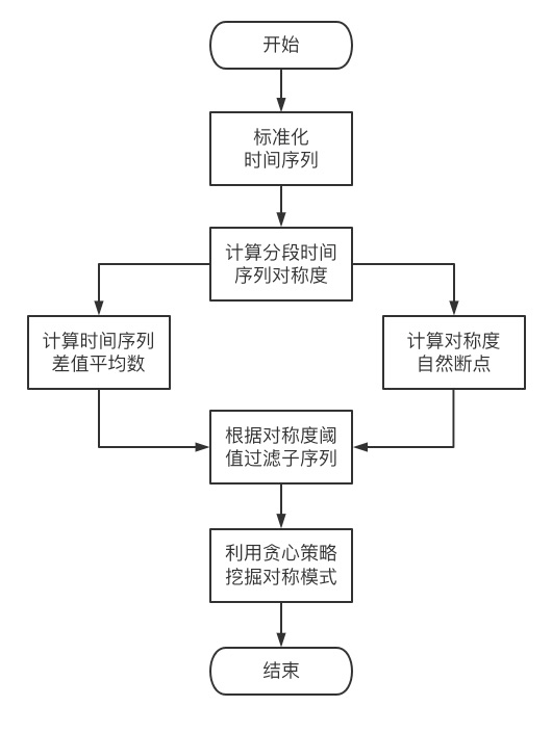
\includegraphics[width=0.86\linewidth]{algorithm_process.png}
  \caption{时间序列对称模式挖掘流程图}
  \label{fig:algorithm_process}
\end{figure}